\documentclass[]{report}
\usepackage{lmodern}
\usepackage{amssymb,amsmath}
\usepackage{ifxetex,ifluatex}
\usepackage{fixltx2e} % provides \textsubscript
\ifnum 0\ifxetex 1\fi\ifluatex 1\fi=0 % if pdftex
  \usepackage[T1]{fontenc}
  \usepackage[utf8]{inputenc}
\else % if luatex or xelatex
  \ifxetex
    \usepackage{mathspec}
  \else
    \usepackage{fontspec}
  \fi
  \defaultfontfeatures{Ligatures=TeX,Scale=MatchLowercase}
\fi
% use upquote if available, for straight quotes in verbatim environments
\IfFileExists{upquote.sty}{\usepackage{upquote}}{}
% use microtype if available
\IfFileExists{microtype.sty}{%
\usepackage{microtype}
\UseMicrotypeSet[protrusion]{basicmath} % disable protrusion for tt fonts
}{}
\usepackage[unicode=true]{hyperref}
\hypersetup{
            pdftitle={Rapport sur l'algorithme de calcul d'Ensemble dominant connexe minimal présenté dans l'article On greedy construction of connected dominating sets in wireless networks de Li, Thai, Wang, Yi, Wan, Du, Tong, Bin, Zao, Wun, Zhou, 2005 (1).},
            pdfauthor={Darius Mercadier Jordi Bertran de Balanda},
            pdfborder={0 0 0},
            breaklinks=true}
\urlstyle{same}  % don't use monospace font for urls
\usepackage{listings}
\usepackage{graphicx,grffile}
\makeatletter
\def\maxwidth{\ifdim\Gin@nat@width>\linewidth\linewidth\else\Gin@nat@width\fi}
\def\maxheight{\ifdim\Gin@nat@height>\textheight\textheight\else\Gin@nat@height\fi}
\makeatother
% Scale images if necessary, so that they will not overflow the page
% margins by default, and it is still possible to overwrite the defaults
% using explicit options in \includegraphics[width, height, ...]{}
\setkeys{Gin}{width=\maxwidth,height=\maxheight,keepaspectratio}
\IfFileExists{parskip.sty}{%
\usepackage{parskip}
}{% else
\setlength{\parindent}{0pt}
\setlength{\parskip}{6pt plus 2pt minus 1pt}
}
\setlength{\emergencystretch}{3em}  % prevent overfull lines
\providecommand{\tightlist}{%
  \setlength{\itemsep}{0pt}\setlength{\parskip}{0pt}}
\setcounter{secnumdepth}{5}
% Redefines (sub)paragraphs to behave more like sections
\ifx\paragraph\undefined\else
\let\oldparagraph\paragraph
\renewcommand{\paragraph}[1]{\oldparagraph{#1}\mbox{}}
\fi
\ifx\subparagraph\undefined\else
\let\oldsubparagraph\subparagraph
\renewcommand{\subparagraph}[1]{\oldsubparagraph{#1}\mbox{}}
\fi

% set default figure placement to htbp
\makeatletter
\def\fps@figure{htbp}
\makeatother

\usepackage[utf8]{inputenc}

% Listing formatting
\lstset{
  basicstyle=\ttfamily,
  breaklines=true,
  postbreak=\raisebox{0ex}[0ex][0ex]{\ensuremath{\hookrightarrow\space}},
  mathescape
}

\title{Rapport sur l'algorithme de calcul d'Ensemble dominant connexe minimal
présenté dans l'article \emph{On greedy construction of connected
dominating sets in wireless networks} de Li, Thai, Wang, Yi, Wan, Du,
Tong, Bin, Zao, Wun, Zhou, 2005 (1).}
\author{Darius Mercadier \and Jordi Bertran de Balanda}
\date{}

\begin{document}
\maketitle

{
\setcounter{tocdepth}{2}
\tableofcontents
}
\newpage

\section{Introduction}\label{introduction}

Un ensemble dominant d'un graphe \emph{G} = (\emph{S}, \emph{A}) est un
sous-ensemble \emph{D} de \emph{S} tel que pour toute arrête \emph{uv}
\(\in\) \emph{A}, \emph{u} \(\in\) \emph{D} ou \emph{v} \(\in\)
\emph{D}. Le problème consistant à trouver un ensemble dominant connexe
de taille minimal (MCDS) est NP-Difficile. Dans ce rapport, nous
étudierons l'algortihme \emph{S-MIS} présenté dans \emph{On greedy
construction of connected dominating sets in wireless networks} de Li,
Thai, Wang, Yi, Wan, Du, Tong, Bin, Zao, Wun, Zhou, 2005, qui propose un
Schema d'approximation en temps polynomial (PTAS) donnant une
\emph{(4.8+ln(5))}-approximation de la solution optimale. Nous
commenceront par présenter l'algorithme, puis présenteront les résultats
expérimentaux obtenus, que nous compareront avec d'autres algorithmes de
résolution de ce problème.

Plus précisémment, nous étudieront cette algorithme dans le contexte des
graphes géométriques. Ceux-ci sont composés d'un ensemble de sommets
\emph{S} et d'arrêtes \emph{A} telles que \emph{uv} \(\in\) \emph{A} si
et seulement si \emph{distance(u,v)} \(\leq\) \emph{k}, \emph{k} étant
un seuil fixe. Nous présenteront également les générateurs aléatoires
utilisés pour générer les graphes de tests.

\section{Présentation de
l'algorithme}\label{pruxe9sentation-de-lalgorithme}

L'algorithme \emph{S-MIS} consiste en deux étapes : le calcul d'un
\emph{Maximum Independent Set} (MIS), puis le calcul du MCDS.

Le papier présentant l'algorithme \emph{S-MIS} ne présente pas
d'algorithme permettant le calcul du MIS, mais suggère deux approches de
calcul (2,3). Nous avons donc implémenté l'algorithme de Wan, Alzoubi et
Frieder (3).

\subsection{Calcul du MIS}\label{calcul-du-mis}

Un ensemble indépendant dans un graphe \emph{G} = (\emph{S}, \emph{A})
est un sous-ensemble \emph{D} de \emph{S} tel que pour tout \emph{u}
\(\in\) \emph{D} et \emph{v} \(\in\) \emph{D}, \emph{uv} \(\notin\)
\emph{A}. Le problème de calculer un ensemble indépendant maximum est
NP-difficile. C'est donc sur une \(\alpha\)-approximation que nous avons
implémenté.\\
Le MIS nécessaire au calcul du MCDS avec l'algorithme S-MIS doit de plus
satisfaire une condition supplémentaire : pour tout \emph{u} \(\in\)
\emph{D}, il doit exister \emph{w} \(\in\) \emph{S} tel qu'il existe
\emph{v} \(\in\) \emph{D}, \emph{v} \(\neq\) \emph{u} tel que \emph{uw}
\(\in\) \emph{A} et \emph{vw} \(\in\) \emph{A}. Moins formellement, cela
signifie qu'entre deux points apparetenant au MIS, il doit y avoir un et
un seul point n'appartenant pas au MIS.

\begin{figure}
\centering
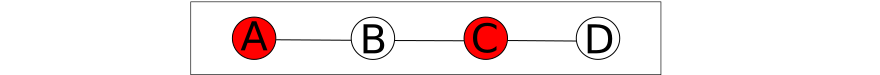
\includegraphics{img/fig1.png}
\caption{Un MIS valide comme base de l'algorithme S-MIS}
\end{figure}

\begin{figure}
\centering
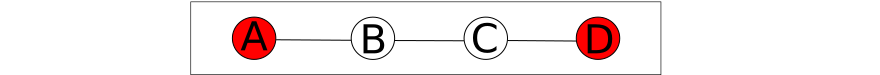
\includegraphics{img/fig2.png}
\caption{Un MIS invalide comme base de l'algorithme S-MIS}
\end{figure}

Les figures 1 et 2 montrent toutes les deux des MIS : tous les sommets
sont soit dans le MIS soit ont un voisin dans le MIS, et aucun sommet du
MIS n'a de voisin dans le MIS. Cependant, dans le second, les deux
sommets du MIS sont séparés d'une distance de deux sommets tandis qu'il
ne sont séparés que d'un sommet dans le premier. Par conséquent, seule
la figure 1 représente un MIS valide comme base de l'algorithme S-MIS.

\subsubsection{Implémentation de l'algorithme de calcul du
MIS}\label{impluxe9mentation-de-lalgorithme-de-calcul-du-mis}

L'algorithme utilisé pour calculer le MIS se base sur un système de
couleur pour différencier les points non-visités (blancs) des points
appartenant au MIS (noirs) et des points n'appartenant pas au MIS
(bleus) : on part d'un point au hasard du graphe, que l'on marque noir
(il est le premier point du MIS). On marque tous ses voisins bleus (il
ne peuvent pas appartenir au MIS). Puis on ajoute les voisins des
voisins qui sont encore blancs à la liste des points potentiellement
dans le MIS. On retire le premier point de cette liste et on réitère le
processus tant qu'il reste des points à examiner.

De manière plus pratique, le pseudo-code de cet algorithme est le
suivant :

\begin{lstlisting}
def MIS ( G = (V,E) ) :
  MIS = []
  for (p : V) :                     # Initializing the colors.
    p.color = White
  
  Stack = [V.pop]
  while (Stack.notEmpty) :
    current = Stack.pop
    if (current.color == Blue) :    # Already covered
      continue
    current.color = Black           # Adding it to the MIS
    MIS.add(current)
    
    for (p : current.neighbors) :
      p.color == Blue               # Marking the neighbors as covered
  
    for (p : current.neighbors) :
      for (q : p.neighbors) :
        if (q.color == White) :     # Adding the neighbors of the neighbors
          Stack.add(q)              #  to the potential points of the MIS.

  return MIS
  
\end{lstlisting}

\subsubsection{Complexité du calcul du
MIS}\label{complexituxe9-du-calcul-du-mis}

On note \emph{n}=\textbar{}\emph{S}\textbar{}, et
\emph{m}=\textbar{}\emph{E}\textbar{}.

\textbf{Initialisation} :\\
Initialiser les couleurs des sommets requière un unique parcours des
sommets, en temps linéaire en la taille de \emph{S} :
\lstinline!O(n)!.\\
Pour des questions d'optimisation, on précalculera lors de
l'initialisation une table d'association point-voisins qui a chaque
point associera ses voisins. Cette opération est réalisable en
\lstinline!O(n*m)!), et permet de réaliser l'opération
\lstinline!neihbors! en \lstinline!O(1)!.

\textbf{Boucle principale} :\\
Le pseudo-code précédemment donné est une version simplifié de
l'algorithme réel pour des raisons de lisibilité, en particulier, dans
une vrai implémentation un point n'est ajouté à la stack que si il n'y
est pas déjà et si il est blanc. En tenant compte de cette condition, et
en constatant qu'il y a autant d'itération de la boucle principale qu'il
y a d'éléments qui sont ajoutés dans la stack lors de l'execution de
l'algorithme, et vu qu'un sommet blanc enlevé de la Stack est marqué
noir, on en conclue que le nombre d'itéreation de cette boucle est borné
par \emph{n}.\\
On a expliqué précédemment que l'opération \lstinline!neighbors! est
réalisable en temps constant. Le nombre de voisins d'un points cependant
est uniquement bornée par \emph{m}. Par conséquent la boucle parcourant
les voisins des voisins a une complexité en \lstinline!O(m*m)!.\\
La complexité de la boucle principale est donc \lstinline!O(n*m*m)!.

Il convient cependant de noter que dans les instances traitées, cette
limite est une sur-approximation très large. En effet, les graphes étant
géométriques, la distribution des sommets aléatoire et uniforme, et le
seuil \emph{k} très inférieur à la distance entre les extrèmes du
domaine de définition des sommets, le nombre d'arrête par sommets sera
très inférieur à \emph{m}.\\
Par conséquent, une complexité plus réaliste serait de l'ordre de
\lstinline!O(n*m)!. (Celà revient à supposer que le nombre d'arrêtes par
sommets est de l'ordre de \(\sqrt{m}\); ce chiffre dépend en réalité de
la quantité de sommets, de l'air de la surface dans laquelle ils sont,
et de l'uniformité de leur répartition. Dans nos test, le nombre
d'arrêtes par sommets est en effet bien plus proche de \(\sqrt{m}\) que
de \emph{m}).

\subsection{Calcul du S-MIS : algorithme de Li et
al.}\label{calcul-du-s-mis-algorithme-de-li-et-al.}

\subsubsection{Principe de l'algorithme}\label{principe-de-lalgorithme}

L'algorithme se base sur un Lemme inhérent à la manière dont le MIS est
construit : il faut au maximum ajouter un point pour connecter deux
points. (cf les figures 1 et 2).\\
Informellement, à partir de ce Lemme, le principe de l'algorithme est de
regrouper des clusters de sommets de manières greedy : on ajoute un à un
les points qui permettent de regrouper le maximum de clusters.\\
L'algorithme utilise un système de couleurs pour déterminer les points
apartenant au MCDS car ils appartiennent au MIS (black) ou car on les y
a rajoutés (blue), et ceux dont le status est encore à déterminer
(grey). Les ``clusters'' de sommets à reliés sont appelés
\emph{black-blue component} (car ils sont induits par des points bleus
et noirs conjoints, en ignorant les connexions entre sommets bleus).
Afin de les relier, on trouve les sommets gris qui sont voisins du plus
de points noirs de différents clusters possible (cette affirmation est
légèrement inexacte car \emph{du plus} est en réalité \emph{5 ou plus},
puis \emph{4}, puis \emph{3}, \emph{2} et finallement \emph{1}, car en
effet, tester toutes les possibilités reviendrait à rajouter un facteur
\emph{m} dans l'algorithme alors qu'en tester \emph{5} ne fait
qu'ajouter une constante). C'est cette partie de l'algorithme qui est
greedy : on ajoute les points qui sur le moment semble aider au maximum
a rendre le MIS connexe.

Le pseudo-code est le suivant :

\begin{lstlisting}
# Params : MIS, the MIS obtained with the previously described method,
#          UDG, the graph from which the CDS should be returned.
    
def AlgorithmA (MIS, UDG) : 
  # Initialization
  for (p $\in$ MIS) :
    p.color = black
  for (p $\in$ UDG and p $\notin$ MIS) :
    p.color = grey
    
  # Main loop
  for (i in 5,4,3,2) :
    if ($\exists$ p $\in$ UDG | p.color = grey and p is adjacent to at least i black nodes in different black-blue compoments ) :
      # Then we choose p to connect those different black-blue components :
      p.color = blue
      
  return { p $\in$ UDG | p.color = blue }
      
  # The S-SMIS is then: MIS $\cup$ AlgorithmA(MIS,UDG) 
\end{lstlisting}

\subsubsection{Analyse de la
complexité}\label{analyse-de-la-complexituxe9}

\paragraph{Complexité spatiale}\label{complexituxe9-spatiale}

Premier point, toutes les opérations de l'algorithme se font \emph{en
place}, c'est à dire sans créer de nouvelles structures, mais uniquement
en travaillant sur les couleurs des sommets. Par conséquent, l'espace
mémoire nécessaire à cet algorithme est uniquement l'espace utilisé pour
stocker le graphe, linéaire en le nombre de sommets.\\
Quelques structures de données supplémentaires peuvent cependant
s'avérer utiles, par exemple pour stocker les \emph{black-blue
components}, et pour accéder aux voisins de chaque noeuds, mais l'espace
occupé restera cependant en \lstinline!O(n)!.

\paragraph{Complexité temporelle}\label{complexituxe9-temporelle}

\section{Performances}\label{performances}

\subsection{Méthode d'évalutation des
performances}\label{muxe9thode-duxe9valutation-des-performances}

Les données obtenues dans cette section sont des moyennes du calcul de
S-MIS sur des graphes générés aléatoirement avec abscisses et ordonnées
des points du graphe choisies uniformément. Nous prenons 500
échantillons par mesure pour pallier aux éventuels cas pathologiques de
graphes, qui arrivent surtout avec des tailles de graphes faibles
(\(\leq\) 250 points).

Ceci a pour conséquence de créer un graphe bien moins `centré' que ceux
rendus disponibles par \lstinline!supportGUI!. En conséquence
l'évaluation est moins adaptée à des réseaux qui seraient centralisés
autour d'un pôle.

Nous distinguons 3 paramètres sur les points en entrée qui peuvent
influer sur la performance des algorithmes de calcul d'un ensemble
dominant connexe.

\begin{enumerate}
\def\labelenumi{\arabic{enumi}.}
\tightlist
\item
  La densité du nuage de points par rapport à leur fourchette d'abscisse
  et d'ordonnées
\item
  La valeur du seuil associé au graphe géométrique
\item
  La taille du nuage de points à traiter, à densité égale et seuil
  correspondant
\end{enumerate}

Afin de ne pas causer de changement involontaire de l'un des paramètres
lors de l'analyse d'un autre, nous modifions les paramètres annexes.

\subsection{Taille du graphe
géométrique}\label{taille-du-graphe-guxe9omuxe9trique}

\subsubsection{Densité et forme du
graphe}\label{densituxe9-et-forme-du-graphe}

On cherche ici à examiner l'impact de la seule augmentation de la taille
du graphe sur les performances de l'algorithme. De manière à préserver
le nombre moyen de voisins d'un noeud, on cherche à contrôler la
`densité' du graphe en variant les plages de valeurs d'abscisses et
d'ordonnées disponible pour respecter:

\[ d = \frac{n}{r^2}\]

avec \(d\) la densité du nuage de points, \(n\) sa taille et \(r\) le
nombre de valeurs possibles pour les coordonnées d'un point.

\subsubsection{Résultat}\label{ruxe9sultat}

\begin{lstlisting}
![Runtime de S-MIS en fonction de la taille du graphe](img/size.png)
\end{lstlisting}

Nous appelons `densité du graphe' la densité du nuage de points initial
réduit aux noeuds des composantes connexes du graphe géométrique.

La densité du graphe peut être variée de deux façons différentes:

\begin{enumerate}
\def\labelenumi{\arabic{enumi}.}
\tightlist
\item
  par une variation du seuil du graphe géométrique, qui a surtout pour
  effet de rendre le graphe plus faiblement connexe mais qui n'élimine
  pas forcément beaucoup de noeuds du graphe
\item
  par une augmentation de la densité réelle de noeuds, c'est-à-dire par
  une réduction de la plage des abscisses et ordonnées des points du
  graphe à taille du nuage de points fixe, ou par une augmentation de la
  taille du nuage de points à seuil approprié et plage de valeurs fixes.
\end{enumerate}

Nous choisissons de modifier la taille du nuage de points, et nous
examinons la qualité de l'ensemble dominant connexe ainsi que le temps
moyen pris pour le générer. De manière à ne pas varier la connexité du
graphe, nous calculons à partir du seuil de départ un seuil approprié
pour chaque valeur présentée ici.

\begin{lstlisting}
![Runtime de S-MIS en fonction de la densite du graphe](img/density.png)
\end{lstlisting}

\subsection{Connexité du graphe
géométrique}\label{connexituxe9-du-graphe-guxe9omuxe9trique}

Nous évaluons ici l'impact de la connexité du graphe sur les
performances de l'algorithme S-MIS. À tailles de nuage de point égales,
nous comparons les impacts de modifications de seuil du graphe
géométrique. Nous nous attendons à ce que la performance en temps de
l'algorithme varie en fonction directe de ce seuil, puisqu'intuitivement
réduire la connexité du graphe réduit non seulement le nombre de noeuds
à traiter, mais aussi le nombre de composantes indiquant les chemins
connexes potentiels que l'algorithme impose de recalculer.

\begin{figure}
\centering
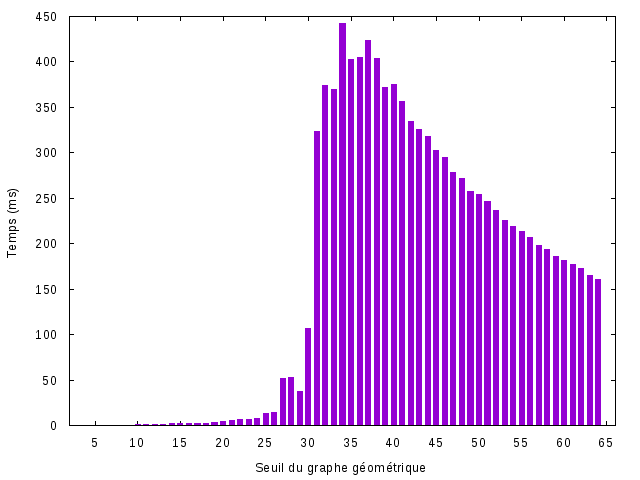
\includegraphics{img/connex.png}
\caption{Runtime de S-MIS en fonction de la connexite du graphe, avec
une taille de nuage fixe de \(800*800\)}
\end{figure}

On remarque que le comportement de l'algorithme n'est pas monotone. En
effet, un graphe très fortement connexe élimine très vite une forte
quantité de noeuds des itérations suivantes de l'algorithme, là où un
graphe moins connexe conserve une quantité importante de noeuds pour les
itérations suivantes.

\section{Références}\label{ruxe9fuxe9rences}

\begin{enumerate}
\def\labelenumi{\arabic{enumi}.}
\tightlist
\item
  Yingshu Li, My T. Thai, Feng Wang, Chih-Wei Yi, Peng-Jun Wan and
  Ding-Zhu Du, On greedy construction of connected dominating sets in
  wireless networks, 2005.
\item
  Cadei M, Cheng MX, Cheng X, Du D-Z. Connected domination in ad hoc
  wireless networks. In Proceedings of the 6th International Conference
  on Computer Science and Informatics (CS\&I'2002), Durham, NC, USA,
  March, 2002.
\item
  Wan P-J, Alzoubi KM, Frieder O. Distributed construction of connected
  dominating set in wireless ad hoc networks. In Proceedings of IEEE
  Infocom 2002, New York, NY, USA, June 2002.
\end{enumerate}

\end{document}
